% !TEX program = lualatex
\documentclass[12pt,a4paper]{article}
\usepackage{fontspec}
\setmonofont{Latin Modern Mono}
\usepackage{xcolor}
\usepackage{listings}
\usepackage{geometry}
\usepackage{fancyhdr}
\usepackage{hyperref}
\usepackage{graphicx}
\geometry{margin=1in}
\usepackage{multicol}

% -------------------------------
% SOLUTION TOGGLE
% -------------------------------
\newif\ifshowsolutions
\showsolutionstrue 
% \showsolutionsfalse

% -------------------------------
% Header and Footer Configuration
% -------------------------------
\pagestyle{fancy}
\fancyhf{}
\lhead{Lab Final}
\rhead{CSE 4308: DBMS Lab}
\cfoot{\thepage}
\setlength{\headwidth}{\textwidth}

% -------------------------------
% Code Listing Style
% -------------------------------
\definecolor{codegreen}{rgb}{0,0.6,0}
\definecolor{codegray}{rgb}{0.5,0.5,0.5}
\definecolor{codepurple}{rgb}{0.58,0,0.82}
\definecolor{backcolour}{rgb}{0.95,0.95,0.92}

\lstdefinestyle{mystyle}{
    backgroundcolor=\color{backcolour},
    commentstyle=\color{codegreen},
    keywordstyle=\color{magenta},
    numberstyle=\tiny\color{codegray},
    stringstyle=\color{codepurple},
    basicstyle=\ttfamily\footnotesize,
    breaklines=true,
    captionpos=b,
    keepspaces=true,
    numbers = none,
    numbersep=5pt,
    tabsize=2,
    frame=single,
    columns=fullflexible,
    showspaces=false,
    showstringspaces=false,
    showtabs=false
}

\lstset{style=mystyle}

% Images: found next to this file (local compile_labs.sh) or via the
% lab folder when compiled from the project root (Overleaf).
\graphicspath{{lab_14_final/}}

\begin{document}

% --------------------------------------------------------------
% TITLE PAGE
% --------------------------------------------------------------
\begin{titlepage}
    \centering
    \vspace*{2\baselineskip}

    \rule{14cm}{2pt}\vspace*{-0.8\baselineskip}\vspace*{1.5pt}
    \rule{14cm}{0.5pt}\vspace{2\baselineskip}

    {\Huge\bfseries\scshape Lab Final\par}
    \vspace{3mm}
    {\Large }
    \vspace{3mm}

    \rule{14cm}{0.5pt}\vspace*{-0.7\baselineskip}\vspace{2.5pt}
    \rule{14cm}{2pt}

    \vspace{2\baselineskip}

    {\Large\bfseries CSE 4308\par}
    \vspace{1\baselineskip}
    {\large DATABASE MANAGEMENT SYSTEMS LAB\par}

    \vfill
    {\normalsize Prepared by:\\ Samnun Azfar, Jr. Lecturer, CSE\\ Samia Nawsheen, Jr. Lecturer, CSE\par}
    {\normalsize Academic Year: AY25-26\par}
\end{titlepage}

\newpage

% ==============================================================
\section{Lab Final}


\begin{enumerate}
% ==============================================================1
\item Write a query that returns customer\_id, first\_name,
last\_name, and the length of their email address.
Only include customers whose email length is greater than 25 characters.
Order by email length in descending order.

\ifshowsolutions
\begin{lstlisting}[language=SQL]
SELECT customer_id,
       first_name,
       last_name,
       LENGTH(email) AS email_length
FROM customer
WHERE LENGTH(email) > 25
ORDER BY email_length DESC;
\end{lstlisting}
\fi
% ==============================================================2
\item Identify customers who have made at least 20 payments with an average payment amount above \$5.00. Show the customer's first and last name, the total number of payments made, and their average payment amount.
\ifshowsolutions
\begin{lstlisting}[language=SQL]
SELECT 
    c.first_name, 
    c.last_name, 
    COUNT(p.payment_id) AS total_payments, 
    ROUND(AVG(p.amount), 2) AS average_payment
FROM customer c
JOIN payment p ON c.customer_id = p.customer_id
GROUP BY c.customer_id, c.first_name, c.last_name
HAVING COUNT(p.payment_id) >= 20 
   AND AVG(p.amount) > 5.00
ORDER BY average_payment DESC;
\end{lstlisting}
\fi

% ==============================================================3
\item Write a query that lists the actor\_id, first\_name, last\_name, and the total number of films for each actor. Only include actors who have appeared in more films than the overall average number of films per actor. Order the results by film count in descending order.

\ifshowsolutions
\begin{lstlisting}[language=SQL]
SELECT a.actor_id,
       a.first_name,
       a.last_name,
       COUNT(fa.film_id) AS film_count
FROM actor a
JOIN film_actor fa ON a.actor_id = fa.actor_id
GROUP BY a.actor_id, a.first_name, a.last_name
HAVING COUNT(fa.film_id) > (
    SELECT AVG(actor_counts.f_count)
    FROM (
        SELECT COUNT(film_id) AS f_count
        FROM film_actor
        GROUP BY actor_id
    ) AS actor_counts
)
ORDER BY film_count DESC;
\end{lstlisting}
\fi

% ==============================================================4
\item Write a query that lists customers whose total spending
is greater than the average spending of customers
within the same store.
Show store\_id, customer\_id, and total\_spent.

\ifshowsolutions
\begin{lstlisting}[language=SQL]
SELECT c.store_id,
       c.customer_id,
       SUM(p.amount) AS total_spent
FROM customer c
JOIN payment p ON p.customer_id = c.customer_id
GROUP BY c.store_id, c.customer_id
HAVING SUM(p.amount) >
       (
           SELECT AVG(store_total)
           FROM (
               SELECT SUM(p2.amount) AS store_total
               FROM customer c2
               JOIN payment p2 ON p2.customer_id = c2.customer_id
               WHERE c2.store_id = c.store_id
               GROUP BY c2.customer_id
           ) sub
       )
ORDER BY c.store_id, total_spent DESC;
\end{lstlisting}
\fi
% 5
\item Write an anonymous PL/pgSQL block that calculates and sequentially prints the Fibonacci sequence up to the Nth number. The sequence starts with 0 and 1, and every subsequent number is the sum of the previous two. The first 10 numbers of the Fibonacci sequence are: 0, 1, 1, 2, 3, 5, 8, 13, 21, 34. 
\ifshowsolutions
\begin{lstlisting}[language=SQL]
DO $$
DECLARE
    n INT := 10;
    a INT := 0;
    b INT := 1;
    temp INT;
BEGIN
    RAISE NOTICE 'Printing the first % Fibonacci numbers:', n;
    
    FOR i IN 1..n LOOP
        RAISE NOTICE '%', a;
        
        -- Calculate the next number in the sequence
        temp := a + b;
        
        -- Shift the values forward for the next iteration
        a := b;
        b := temp;
    END LOOP;
END $$;
\end{lstlisting}
\fi
\item Write an anonymous PL/pgSQL block that prints all film title, description and description length where the film's description mentions a "Moose" and a "Robot" or a "Moose" and a "Dentist" anywhere in the sentence, and the description length is strictly greater than 20 characters. Order the output by description length in descending order.

\ifshowsolutions
\begin{lstlisting}[language=SQL]
DO $$
DECLARE
    rec RECORD;
BEGIN
    FOR rec IN
        SELECT film_id, title, length, description
        FROM film
        WHERE LENGTH(description) > 20
          AND description LIKE '%Moose%' 
          AND (description LIKE '%Robot%' OR description LIKE '%Dentist%')
        ORDER BY length DESC, film_id
    LOOP
        RAISE NOTICE 'Film %: % (Length: %) | Desc: %',
            rec.film_id, rec.title, rec.length, rec.description;
    END LOOP;
END $$;
\end{lstlisting}
\fi
% 6
% \item Write an anonymous block that takes a film id (e.g., 1) and prints whether the film is: 
% 'Short' (length < 60),
% 'Medium' (60–120),
% or 'Long' (> 120).

% \ifshowsolutions
% \begin{lstlisting}[language=SQL]
% DO $$
% DECLARE
%     v_film_id INT := 1;
%     v_title TEXT;
%     v_length INT;
% BEGIN
%     SELECT title, length
%     INTO v_title, v_length
%     FROM film
%     WHERE film_id = v_film_id;

%     IF NOT FOUND THEN
%         RAISE NOTICE 'Film % not found', v_film_id;
%         RETURN;
%     END IF;

%     IF v_length < 60 THEN
%         RAISE NOTICE 'Film % (% minutes) -> Short',
%             v_title, v_length;
%     ELSIF v_length <= 120 THEN
%         RAISE NOTICE 'Film % (% minutes) -> Medium',
%             v_title, v_length;
%     ELSE
%         RAISE NOTICE 'Film % (% minutes) -> Long',
%             v_title, v_length;
%     END IF;
% END $$;
% \end{lstlisting}
% \fi

% % 7
% \item Write an anonymous block that takes a category id (e.g., 1) and prints: the category name and the number of films in that category.

% \ifshowsolutions
% \begin{lstlisting}[language=SQL]
% DO $$
% DECLARE
%     v_category_id INT := 1;
%     v_name TEXT;
%     v_cnt INT;
% BEGIN
%     SELECT name INTO v_name
%     FROM category
%     WHERE category_id = v_category_id;

%     IF NOT FOUND THEN
%         RAISE NOTICE 'Category % not found', v_category_id;
%         RETURN;
%     END IF;

%     SELECT COUNT(*)
%     INTO v_cnt
%     FROM film_category
%     WHERE category_id = v_category_id;

%     RAISE NOTICE 'Category % (%): % films',
%         v_category_id, v_name, v_cnt;
% END $$;
% \end{lstlisting}
% \fi
% ==============================================================
\item Write a PL/pgSQL function to find the best-selling film of a specific category. The category name will be the input parameter, and the function should return the title of the film that generated the highest total revenue
\ifshowsolutions
\begin{lstlisting}[language=SQL]
CREATE OR REPLACE FUNCTION get_best_selling_film_by_category(p_category_name VARCHAR)
RETURNS VARCHAR
LANGUAGE plpgsql
AS $$
DECLARE
    v_film_title VARCHAR(255);
BEGIN
    SELECT f.title INTO v_film_title
    FROM category c
    JOIN film_category fc ON c.category_id = fc.category_id
    JOIN film f ON fc.film_id = f.film_id
    JOIN inventory i ON f.film_id = i.film_id
    JOIN rental r ON i.inventory_id = r.inventory_id
    JOIN payment p ON r.rental_id = p.rental_id
    WHERE c.name = p_category_name
    GROUP BY f.film_id, f.title
    ORDER BY SUM(p.amount) DESC
    LIMIT 1;

    RETURN v_film_title;
END;
$$;
SELECT get_best_selling_film_by_category('Action') AS best_selling_film;
\end{lstlisting}
\fi

% ==============================================================
\item Create a stored procedure inventory\_availability\_summary to summarize a film's availability in a specific store. It must count total copies, count available copies, and update an input variable with the availability percentage.

\ifshowsolutions
\begin{lstlisting}[language=SQL]
CREATE OR REPLACE PROCEDURE inventory_availability_summary(
    p_film_id INT,
    p_store_id INT,
    INOUT p_avail_pct NUMERIC,
    OUT o_total_copies INT,
    OUT o_available_copies INT
)
LANGUAGE plpgsql
AS $$
DECLARE
    v_rented_copies INT;
BEGIN
    SELECT COUNT(*) INTO o_total_copies
    FROM inventory 
    WHERE film_id = p_film_id AND store_id = p_store_id;

    SELECT COUNT(DISTINCT r.inventory_id) INTO v_rented_copies
    FROM rental r
    JOIN inventory i ON i.inventory_id = r.inventory_id
    WHERE i.film_id = p_film_id AND i.store_id = p_store_id AND r.return_date IS NULL;

    o_available_copies := o_total_copies - v_rented_copies;

    IF o_total_copies = 0 THEN
        p_avail_pct := 0;
    ELSE
        p_avail_pct := ROUND((o_available_copies::NUMERIC * 100.0) / o_total_copies, 2);
    END IF;
END;
$$;

DO $$
DECLARE
    -- Initialize the INOUT parameter
    v_availability_percentage NUMERIC := 0.00; 
    v_total INT;
    v_available INT;
BEGIN
    CALL inventory_availability_summary(
        586,                          -- p_film_id (IN)
        1,                          -- p_store_id (IN)
        v_availability_percentage,  -- p_avail_pct (INOUT)
        v_total,                    -- o_total_copies (OUT)
        v_available                 -- o_available_copies (OUT)
    );

    -- Print the returned values
    RAISE NOTICE 'Total Inventory: %', v_total;
    RAISE NOTICE 'Available for Rent: %', v_available;
    RAISE NOTICE 'Availability: %%%', v_availability_percentage;
END;
$$;
\end{lstlisting}
\fi
% ==============================================================
\item Write a PL/pgSQL function that takes two store IDs, compares their customers' average lifetime spending, and returns a message stating which store is more profitable.
\ifshowsolutions
\begin{lstlisting}[language=SQL]
CREATE OR REPLACE FUNCTION compare_store_profitability(store_a_id INT, store_b_id INT)
RETURNS VARCHAR AS $$
DECLARE
    store_a_avg DECIMAL(10,2);
    store_b_avg DECIMAL(10,2);
    result_msg VARCHAR(255);
BEGIN
    SELECT AVG(customer_total) INTO store_a_avg
    FROM (
        SELECT c.customer_id, SUM(p.amount) AS customer_total
        FROM customer c
        JOIN payment p ON c.customer_id = p.customer_id
        WHERE c.store_id = store_a_id
        GROUP BY c.customer_id
    ) a_totals;

    SELECT AVG(customer_total) INTO store_b_avg
    FROM (
        SELECT c.customer_id, SUM(p.amount) AS customer_total
        FROM customer c
        JOIN payment p ON c.customer_id = p.customer_id
        WHERE c.store_id = store_b_id
        GROUP BY c.customer_id
    ) b_totals;

    store_a_avg := COALESCE(store_a_avg, 0);
    store_b_avg := COALESCE(store_b_avg, 0);

    IF store_a_avg > store_b_avg THEN
        result_msg := 'Store ' || store_a_id || ' is stronger (Avg: $' || ROUND(store_a_avg, 2) || ' vs $' || ROUND(store_b_avg, 2) || ')';
    ELSIF store_b_avg > store_a_avg THEN
        result_msg := 'Store ' || store_b_id || ' is stronger (Avg: $' || ROUND(store_b_avg, 2) || ' vs $' || ROUND(store_a_avg, 2) || ')';
    ELSE
        result_msg := 'Both stores have equal profitability (Avg: $' || ROUND(store_a_avg, 2) || ')';
    END IF;

    RETURN result_msg;
END;
$$ LANGUAGE plpgsql;
\end{lstlisting}
\fi

% \item Create a function that takes a customer ID and returns the number of \textbf{distinct categories} the customer has rented from.

% \ifshowsolutions
% \begin{lstlisting}[language=SQL]
% CREATE OR REPLACE FUNCTION customer_category_count(p_customer_id INT)
% RETURNS INT
% LANGUAGE plpgsql
% AS $$
% DECLARE
%     v_cnt INT;
% BEGIN
%     SELECT COUNT(DISTINCT fc.category_id)
%     INTO v_cnt
%     FROM rental r
%     JOIN inventory i ON i.inventory_id = r.inventory_id
%     JOIN film_category fc ON fc.film_id = i.film_id
%     WHERE r.customer_id = p_customer_id;

%     RETURN COALESCE(v_cnt, 0);
% END;
% $$;

% -- Invocation (example)
% SELECT customer_category_count(1);
% \end{lstlisting}
% \fi

\item Create a function that takes a customer ID and returns the name of the most-rented category for that customer. If the customer has no rentals, return NULL.

\ifshowsolutions
\begin{lstlisting}[language=SQL]
CREATE OR REPLACE FUNCTION top_category_name(p_customer_id INT)
RETURNS TEXT
LANGUAGE plpgsql
AS $$
DECLARE
    v_name TEXT;
BEGIN
    SELECT c.name
    INTO v_name
    FROM rental r
    JOIN inventory i ON i.inventory_id = r.inventory_id
    JOIN film_category fc ON fc.film_id = i.film_id
    JOIN category c ON c.category_id = fc.category_id
    WHERE r.customer_id = p_customer_id
    GROUP BY c.name, c.category_id
    ORDER BY COUNT(*) DESC, c.category_id
    LIMIT 1;

    RETURN v_name; -- NULL if none
END;
$$;

-- Invocation (example)
SELECT top_category_name(1);
\end{lstlisting}
\fi


% % ==============================================================
% \item Create a procedure that moves an inventory item to another store by updating \texttt{inventory.store\_id}. If the inventory ID does not exist, raise an exception.

% \ifshowsolutions
% \begin{lstlisting}[language=SQL]
% CREATE OR REPLACE PROCEDURE transfer_inventory(p_inventory_id INT, p_target_store INT)
% LANGUAGE plpgsql
% AS $$
% BEGIN
%     UPDATE inventory
%     SET store_id = p_target_store
%     WHERE inventory_id = p_inventory_id;

%     IF NOT FOUND THEN
%         RAISE EXCEPTION 'Inventory id % not found', p_inventory_id;
%     END IF;

%     RAISE NOTICE 'Inventory % moved to store %', p_inventory_id, p_target_store;
% END;
% $$;

% -- Invocation (example)
% CALL transfer_inventory(1, 2);
% \end{lstlisting}
% \fi


\end{enumerate}
\newpage
\section{ER Diagram}
\begin{figure}[h]
        \centering
        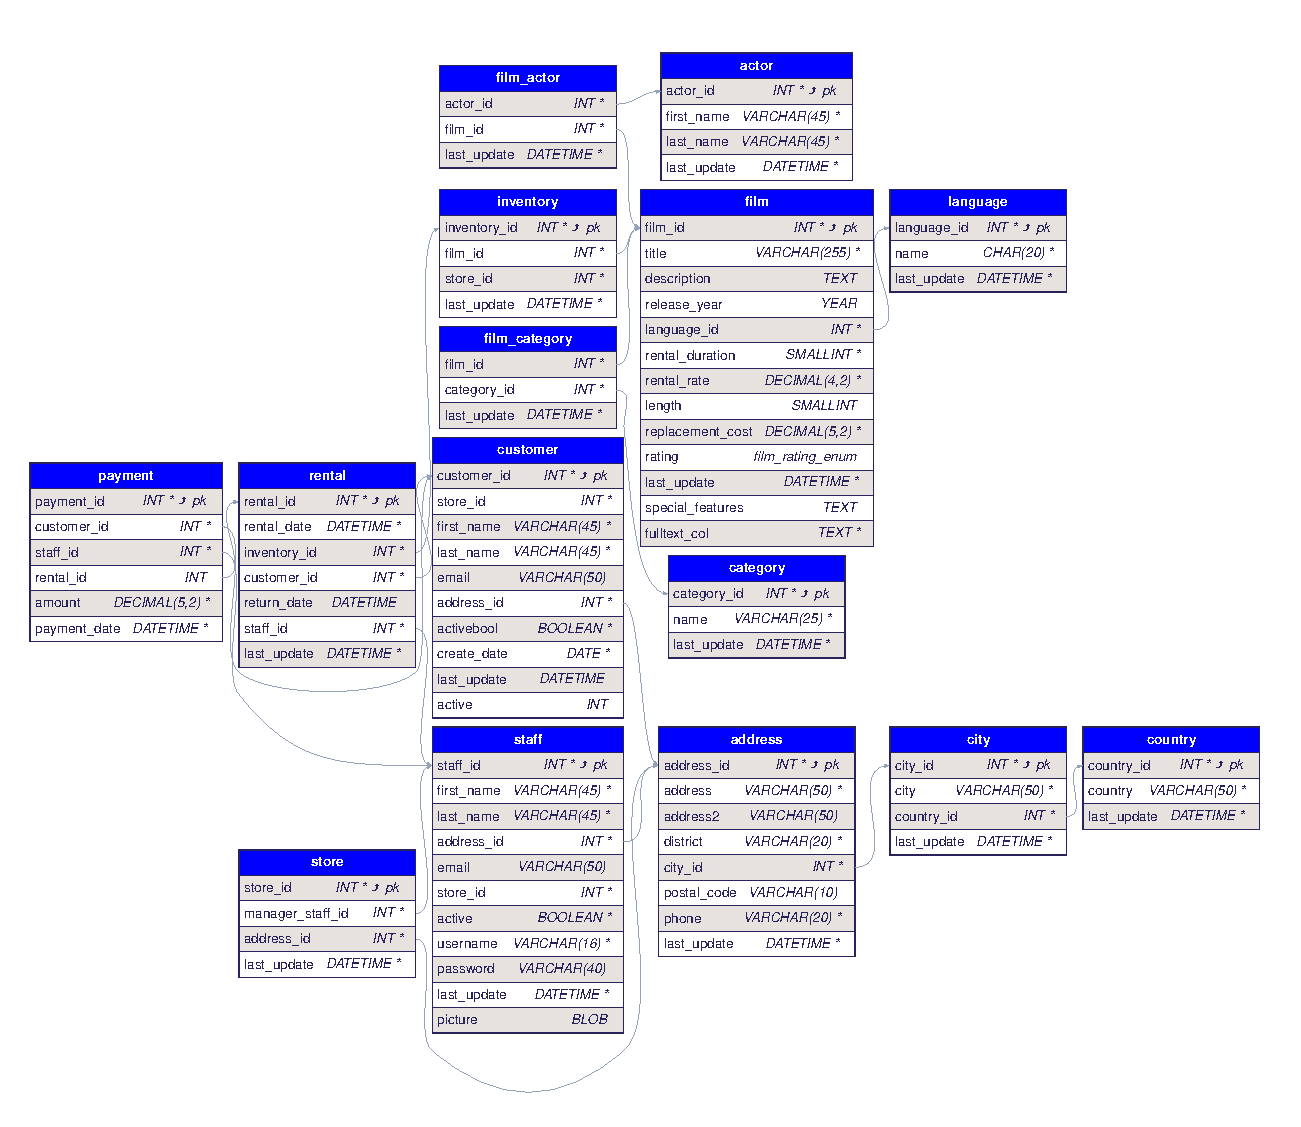
\includegraphics[width=\textheight, height=\textwidth, keepaspectratio, angle=90]{lab_14_schema_cropped.pdf}
\end{figure}

\end{document}